\documentclass[11pt]{article}
\usepackage{fontspec}
\setmainfont{Times New Roman}
\usepackage{amsmath,amssymb}
\usepackage{textcomp}
\usepackage{newunicodechar}
\newunicodechar{⇒}{\ensuremath{\Rightarrow}}
\usepackage{booktabs}
\usepackage{longtable}
\usepackage{array}
\usepackage{multirow}
\usepackage{calc} % for calculating minipage widths
\usepackage{caption}
\captionsetup[table]{skip=6pt}
\newcounter{none} % for unnumbered tables
\usepackage{etoolbox}
\makeatletter
\patchcmd\longtable{\par}{\if@noskipsec\mbox{}\fi\par}{}{}
\makeatother
\providecommand{\tightlist}{%
  \setlength{\itemsep}{0pt}\setlength{\parskip}{0pt}}
\usepackage{graphicx}
\makeatletter
\newsavebox\pandoc@box
\newcommand*\pandocbounded[1]{% scales image to fit in text height/width
  \sbox\pandoc@box{#1}%
  \Gscale@div\@tempa{\textheight}{\dimexpr\ht\pandoc@box+\dp\pandoc@box\relax}%
  \Gscale@div\@tempb{\linewidth}{\wd\pandoc@box}%
  \ifdim\@tempb\p@<\@tempa\p@\let\@tempa\@tempb\fi% select the smaller of both
  \ifdim\@tempa\p@<\p@\scalebox{\@tempa}{\usebox\pandoc@box}%
  \else\usebox{\pandoc@box}%
  \fi%
}
\def\fps@figure{htbp}
\makeatother
\usepackage{float}
\usepackage{caption}
\usepackage[margin=2.4cm]{geometry}
\usepackage{xcolor}
\usepackage[colorlinks=true,linkcolor=Black,urlcolor=Blue,citecolor=Black]{hyperref}
\usepackage{fancyhdr}
\pagestyle{fancy}
\fancyhf{}
\fancyhead[L]{\small\leftmark}
\fancyhead[R]{\small\thepage}
\begin{document}
\section{Verbatim Claim Verification against Retrieval-Associative
Entailment: Deterministic Evidence Provenance for LLM-Assisted
Systematic
Synthesis}\label{verbatim-claim-verification-against-retrieval-associative-entailment-deterministic-evidence-provenance-for-llm-assisted-systematic-synthesis}

\subsection{A head-to-head evaluation of two claim-generation pipelines
over one screened
corpus}\label{a-head-to-head-evaluation-of-two-claim-generation-pipelines-over-one-screened-corpus}

\begin{center}\rule{0.5\linewidth}{0.5pt}\end{center}

\textbf{Manuscript type}: Methods paper \textbf{Manuscript status}:
Final v1.3 for author review and submission (post-D2 submission review)
\textbf{Workspace}: \texttt{workspaces/ai-research-harnesses-trust} ·
domain: AI-assisted research harnesses, 2023--2026 \textbf{All headline
statistics recomputed from committed ledgers}
(\texttt{synthesis/claims.json},
\texttt{synthesis/rag\_baseline/claims.json},
\texttt{literature/screening/final\_reconciled\_decisions.json})

\begin{center}\rule{0.5\linewidth}{0.5pt}\end{center}

\textbf{Authors}

Mouadh Bekhouche\emph{¹ and Soumia Zertal}²

¹² University of Oum El Bouaghi, Algeria

*Contributed equally to this work. ² Corresponding author. Email:
zertal.soumia@univ-oeb.dz

\begin{center}\rule{0.5\linewidth}{0.5pt}\end{center}

\subsection{Abstract}\label{abstract}

\textbf{Background.} Large language models (LLMs) are increasingly
embedded in the systematic-review lifecycle, yet their outputs are not
trustworthy by default. Under realistic deployment constraints, no model
exceeded a citation-existence rate of 0.475 across 17,443 generated
citations {[}1{]}, and without retrieval grounding 78--98\% of cited
papers are fabricated {[}2{]}. Worse, the metrics commonly used to score
synthesized output can be actively misleading: BERTScore {[}3,11{]} and
ROUGE {[}12{]} have been shown to rate factually false conclusions as
semantically equivalent to verified truths {[}3{]}, and BLEU/ROUGE
scores proved ``not meaningful'' against human assessment in a PICO
feasibility study {[}4{]}. The field lacks a \emph{deterministic}
claim-evidence gate --- a pass/fail test that does not itself appeal to
an LLM judge.

\textbf{Methods.} We formalize \textbf{verbatim claim verification}:
each synthesis claim is reduced to an atomic evidence quote, and that
quote is machine-checked against the approved source full text at a
defined glyph-normalized coverage threshold. Matching uses
glyph-normalized text (NFKC; bullet, dash and quote canonicalization;
hyphen-wrap rejoin) through dual-pass sliding character windows (8
characters, step 4) and token 6-grams (6 tokens, step 3), with a pass
threshold of ≥ 0.90 coverage on either metric --- i.e., the verified
quote matches the source at ≥90\% alignment, not byte-for-byte. We
compared this method against a deterministic retrieval-augmented
generation (RAG) baseline over the same corpus --- 239 de-duplicated
records screened by four independent AI screeners (Fleiss' κ = 0.408)
with majority rule and adjudicated deadlock resolution, yielding 58
included studies.

\textbf{Results.} The RAG baseline generated 90 claims (30 per research
question), of which only \textbf{39/90 (43.3\%)} passed its own
snippet-entailment gate (RQ1 11/30 = 36.7\%, 95\% CI 21.9--54.5\%; RQ2
14/30 = 46.7\%, CI 30.2--63.9\%; RQ3 14/30 = 46.7\%, CI 30.2--63.9\%).
Because the gate scores each claim against the retrieval snippet that
produced it, this is a \emph{self-referential, lenient} bar: it
certifies consistency with retrieved context, not presence in an
approved source. It represented only 25 studies (14 in-scope), produced
at least one verified claim for just 8 of the 14 in-scope studies it
covered, cited \textbf{11 studies absent from the included set} --- a
single excluded source supplied 22 of the 90 claims --- and had zero
claims for 44 of the 58 included studies. The verbatim pipeline
generated 510 claims (RQ1 166 / RQ2 132 / RQ3 212; 493 full-text, 17
abstract-only; 57 studies), all of which reached \textbf{≥90\%
glyph-normalized coverage after a tracked repair loop} (v1: 156 failures
→ v4: 11 → final: 0), with fully verified claims for 57 of the 58
included studies. The verification-rate contrast is decisive (one-sided
Fisher exact test on the pooled claim counts, p ≈ 1.3 × 10⁻⁴⁹;
descriptive of effect size, since claims within a pipeline share
generator context). Semantic consensus over the verbatim ledger
(cached-embedding cosine, θ = 0.40) surfaced 95 clusters (16
high-consensus, 7 active debates, 37 unresolved, 35 provisional) versus
20 clusters and zero debates for RAG.

\textbf{Conclusions.} A deterministic, threshold-verified trust gate is
tractable and strictly stronger than retrieval-associative entailment:
the ≥0.90 glyph-normalized coverage criterion on char-window or token
6-gram alignment is re-runnable by any party on every claim. Retrieval
restriction causes both under-coverage and corpus contamination;
full-text reading with quote-level verification removes both and
additionally exposes genuine debate structure. We recommend verbatim
verification as the default provenance gate for LLM-assisted review
destined for peer-reviewed evidence synthesis, with corpus-scope
enforcement as a mandatory precondition.

\textbf{Keywords}: evidence synthesis; retrieval-augmented generation;
verbatim verification; claim provenance; hallucination detection;
systematic review automation

\begin{center}\rule{0.5\linewidth}{0.5pt}\end{center}

\subsection{1. Introduction}\label{introduction}

LLMs are now embedded at nearly every stage of the systematic-review
pipeline --- federated search, title-and-abstract screening, full-text
extraction, and final synthesis. The attraction is obvious: screening
workloads and extraction effort shrink by orders of magnitude, and
narratives that would take a human team months can be produced in hours.
But the same automation that makes this tractable also manufactures a
new class of risks, and the evidence on those risks is consistently
sobering.

The first failure mode is \emph{generation without verification}. Zhao
et al.~{[}1{]} generated 17,443 citations across four models and five
prompting regimes under deployment constraints; no model, under any
condition, exceeded a citation-existence rate of 0.475, and output
remained format-compliant even as the underlying failures grew
twenty-five-fold in the worst conditions. The same study's manual audit
--- agreement 0.63 with human labels --- showed that ``Unresolved''
labels are not benign: 16 of 35 were in fact fabricated. Un-grounded
generation is worse. Asai et al.~{[}2{]} report fabrication rates of
78--98\% for non-retrieval LLMs, most severe in biomedicine, while their
retrieval-grounded OpenScholar-8B produced zero hallucinated papers in
both computer science and biomedicine.

The second, subtler failure mode is \emph{weak verification}. A
synthesis pipeline that scores its own output against a similarity
metric can certify garbage. Ha et al.~{[}3{]} demonstrate that BERTScore
gives nearly identical F1 scores across retrieval workflows and rates
conclusions produced from \emph{negated} (factually inverted) abstracts
as semantically equivalent to correct ones; Schmidt et al.~{[}4{]}
similarly found BLEU/ROUGE results ``not meaningful'' against human
assessment in a PICO extraction study. Retrieval-augmented generation
(RAG) {[}5{]} is the standard mitigation, and it removes the worst of
the \emph{generation} problem --- grounded systems stop inventing
papers. But \emph{grounding is not verification}: a claim can be
entailed by the snippet that produced it while appearing verbatim
nowhere in that snippet or its source, and the retrieval window itself
silently constrains both coverage and scope.

What is missing is a deterministic notion of claim evidence: a pass/fail
judgment defined purely over a quote and an approved source text,
computable by any party on any run, with no LLM judge in the loop. This
paper proposes exactly that primitive and evaluates it head-to-head.

Our contributions are threefold:

\begin{enumerate}
\def\labelenumi{\arabic{enumi}.}
\tightlist
\item
  \textbf{A trust-provenance method} --- corpus-scoped, multi-agent
  full-text claim extraction with deterministic verbatim verification,
  an auditable repair loop, and an append-only audit ledger.
\item
  \textbf{A same-corpus evaluation} --- the verbatim pipeline and a
  deterministic RAG baseline run over the identical 58-study screened
  set, with every statistic recomputed directly from committed ledgers
  rather than drawn from reports.
\item
  \textbf{Deterministic trust metrics} --- verbatim coverage,
  corpus-scope compliance, and consensus structure --- none of which
  depend on an LLM judge.
\end{enumerate}

\subsection{2. Materials and Methods}\label{materials-and-methods}

\subsubsection{2.1 Corpus and screening}\label{corpus-and-screening}

Five scholarly sources were federated in a single pass (OpenAlex,
Semantic Scholar, Crossref, PubMed, arXiv; bioRxiv-track preprints are
captured via PubMed indexing), returning 250 raw hits that were
de-duplicated and hydrated (DOI and normalized-title resolution,
abstract and metadata completion) to \textbf{239 unique verified
records} targeting LLM/agentic review automation, 2023--2026. Four
independent AI screeners (three Gemini instances and one OpenCode-based
agent; identical written screening instructions committed in
\texttt{literature/screening/}, run independently and blind to one
another) scored all records in an agent-in-the-loop protocol against
explicit inclusion criteria. Inter-rater agreement was \textbf{Fleiss' κ
= 0.408} {[}6{]}; on the Landis \& Koch conventions this is ``fair''
agreement {[}10{]}. Majority rule (≥ 3 of 4 votes) resolved 213 records;
the remaining \textbf{26 two-vs-two deadlocks} were adjudicated by a
senior adjudicator. Final: \textbf{58 included / 181 excluded}. All
downstream synthesis was scoped strictly to the 58 included studies.

The corpus is organized around three research questions that structure
the evaluation throughout. \textbf{RQ1} asks about the state of the art
in academic research and literature-review harnesses integrating LLMs
and agentic AI (2023--2026) and the concrete design mechanisms those
harnesses implement for execution provenance, audit trails, and process
reproducibility. \textbf{RQ2} asks what evidence-trust and
academic-integrity mechanisms (citation fact-checking, hallucination
mitigation, retraction checks, risk-of-bias, open-science artifact
verification) are incorporated into modern harnesses. \textbf{RQ3} asks
how such harnesses are empirically evaluated (benchmarks, ablations,
inter-rater reliability, user studies) and what architectural gaps
remain for trustworthy research infrastructure. Screening and reporting
follow the PRISMA 2020 flow structure {[}13{]}; the corpus is
descriptive in nature, so PRISMA-ScR {[}14{]} conventions are applied
where they diverge.

\subsubsection{2.2 Full-text acquisition, extraction, and the scope
decision}\label{full-text-acquisition-extraction-and-the-scope-decision}

Open-Access PDFs were retrieved and converted to YAML-frontmatter
Markdown (64 documents; 3,814 structural AST chunks). Of the 64, 31 cite
arXiv as source and all carry structured DOIs; the remainder are
published-venue preprints or articles, so the corpus spans LaTeX-derived
arXiv text and publisher-rendered text. One decision matters for what
follows: extraction ran \emph{before} final scoping, so 18 of the 64
extractions belong to screened-out studies. The RAG index inherited this
superset --- a design flaw we deliberately did not paper over, because
it is precisely the contamination mechanism the paper measures. The
verbatim pipeline consumed only the 58 included studies (46 with full
text, 12 abstract-only).

\subsubsection{2.3 Verbatim claim
pipeline}\label{verbatim-claim-pipeline}

\textbf{Generation.} Eight parallel agents read the full text of the 46
extracted included papers (7 size-balanced batches, each ≤
\textasciitilde456 KB) plus one agent over the 12 abstract-only papers.
Each claim was written to a canonical 10-field schema (\texttt{rq\_id},
\texttt{claim\_text}, \texttt{citation\_tokens},
\texttt{evidence\_quote}, \texttt{section}, \texttt{stance},
\texttt{evidence\_level}, \texttt{location\_hint}, \texttt{study\_id},
\texttt{entailment}), with every \texttt{evidence\_quote} drawn from the
source text.

\textbf{Verification (\texttt{VerbatimClaimVerifier}).} Every quote is
checked against its source extraction through three deterministic
stages:

\begin{itemize}
\tightlist
\item
  \emph{Normalization} --- NFKC; removal of zero-width spaces and soft
  hyphens; canonicalization of bullets and box glyphs to \texttt{-},
  Unicode dashes (--- -- −) to \texttt{-}, and curly quotes to ASCII;
  hyphenated line-break rejoin
  (\texttt{"sys-\textbackslash{}n\ tem"\ →\ "system"}); whitespace
  collapse.
\item
  \emph{Matching, dual-pass} --- sliding character windows (8
  characters, step 4) and token 6-grams (6 tokens, step 3), both scored
  as the fraction of quote windows present in the source.
\item
  \emph{Pass rule} --- \textbf{max(char-window coverage, token-6-gram
  coverage) ≥ 0.90}.
\end{itemize}

Because both matchers are pure functions of the quote and the source
file, the outcome is reproducible by any party on any run, and failures
can be inspected individually.

\subsubsection{2.4 RAG baseline (comparison
arm)}\label{rag-baseline-comparison-arm}

The baseline used the same corpus through the kit's deterministic
synthesizer: each research question was embedded and the \textbf{top-30
chunks} retrieved from the full 64-document vector store (collection
\texttt{scholar\_docs}, \texttt{all-MiniLM-L6-v2} embeddings {[}7{]}); a
one-way entailment heuristic then scored each generated claim against
its \emph{own supporting snippet} --- the retrieval context, not the
source document. By construction, RAG claims carry no
\texttt{evidence\_quote} field, so no verbatim gate is even expressible
for them; their only verification is snippet entailment. Outputs:
\texttt{synthesis/rag\_baseline/}.

\subsubsection{2.5 Independent recomputation of every
result}\label{independent-recomputation-of-every-result}

For defensibility, each headline statistic in §3 was \textbf{recomputed
directly from committed ledgers} rather than copied from any report, and
the recomputation itself is shipped as a runnable script
(\texttt{scripts/reproduce\_d2\_stats.py}, executed with
\texttt{uv\ run\ python}; requires numpy/scipy only). Verification
statuses were recoded from each RAG claim's \texttt{entailment\_status}
field; corpus-scope compliance by intersecting each pipeline's distinct
\texttt{study\_id} set with the reconciled included set; and
verification rates with Wilson 95\% confidence intervals, contrasted via
a one-sided Fisher exact test on the pooled two-by-two table. The script
asserts each manuscript number against the ledgers and fails loudly on
any mismatch --- so Table 1 and §3.2 are, in effect, audited by
construction rather than by assertion.

\subsubsection{2.6 Consensus and Phase-4 trust
streams}\label{consensus-and-phase-4-trust-streams}

The 510-claim ledger was clustered with cached-embedding cosine
similarity (\texttt{all-MiniLM-L6-v2}, θ = 0.40) into a consensus map
whose clusters were typed high-consensus / active-debate / unresolved /
provisional. Each study additionally received a trust grade (BLOCKED →
UNVERIFIED → WEAK → ADEQUATE → STRONG) from four Phase-4 verification
streams --- retraction status (OpenAlex \texttt{is\_retracted}, Crossref
\texttt{update-to}), open-science DAS/CAS artifact scanning,
conflict-of-interest audit, and QUADAS-2/PROBAST-style risk-of-bias
attestation {[}8{]}{[}9{]}. Every pipeline step was recorded in an
append-only audit journal (69 events).

\subsection{3. Results}\label{results}

\subsubsection{3.1 Head-to-head claim
verification}\label{head-to-head-claim-verification}

The two pipelines display a stark and structurally-grounded contrast
(Table 1, Figure 1).

\textbf{Table 1.} Head-to-head comparison of the two claim-generation
pipelines.

{\def\LTcaptype{none} % do not increment counter
\begin{longtable}[]{@{}
  >{\raggedright\arraybackslash}p{(\linewidth - 4\tabcolsep) * \real{0.2727}}
  >{\raggedleft\arraybackslash}p{(\linewidth - 4\tabcolsep) * \real{0.3636}}
  >{\raggedleft\arraybackslash}p{(\linewidth - 4\tabcolsep) * \real{0.3636}}@{}}
\toprule\noalign{}
\begin{minipage}[b]{\linewidth}\raggedright
Metric
\end{minipage} & \begin{minipage}[b]{\linewidth}\raggedleft
RAG baseline
\end{minipage} & \begin{minipage}[b]{\linewidth}\raggedleft
Verbatim pipeline
\end{minipage} \\
\midrule\noalign{}
\endhead
\bottomrule\noalign{}
\endlastfoot
Claims generated & 90 (30 per RQ) & 510 (RQ1 166 / RQ2 132 / RQ3 212) \\
Verification pass rate & 39/90 = \textbf{43.3\%} (RQ1 11/30, RQ2 14/30,
RQ3 14/30) & \textbf{510/510 = 100\%} \\
Distinct studies represented & 25 (14 in-scope) & 57 \\
In-scope studies with zero claims & \textbf{44 of 58} & 0 of 57 \\
Citations to non-included studies & \textbf{11} (SCI-000184 alone: 22/90
claims) & 0 \\
Corpus-scope compliance & 64 indexed docs, 18 screened-out & 58 included
only \\
Consensus clusters (θ = 0.40) & 20 (2 HC / 0 debates / 3 unresolved / 15
provisional) & 95 (16 HC / \textbf{7 debates} / 37 unresolved / 35
provisional) \\
\end{longtable}
}

\textbf{Figure 1.} Head-to-head verification coverage: the RAG baseline
passes 39/90 claims (43.3\%) under its own snippet-entailment gate and
represents 25 studies (14 in-scope); the verbatim pipeline passes
510/510 at ≥0.90 glyph-normalized coverage across 57/58 included
studies, leaving 44/58 included studies invisible to the baseline.

\begin{figure}
\centering
\pandocbounded{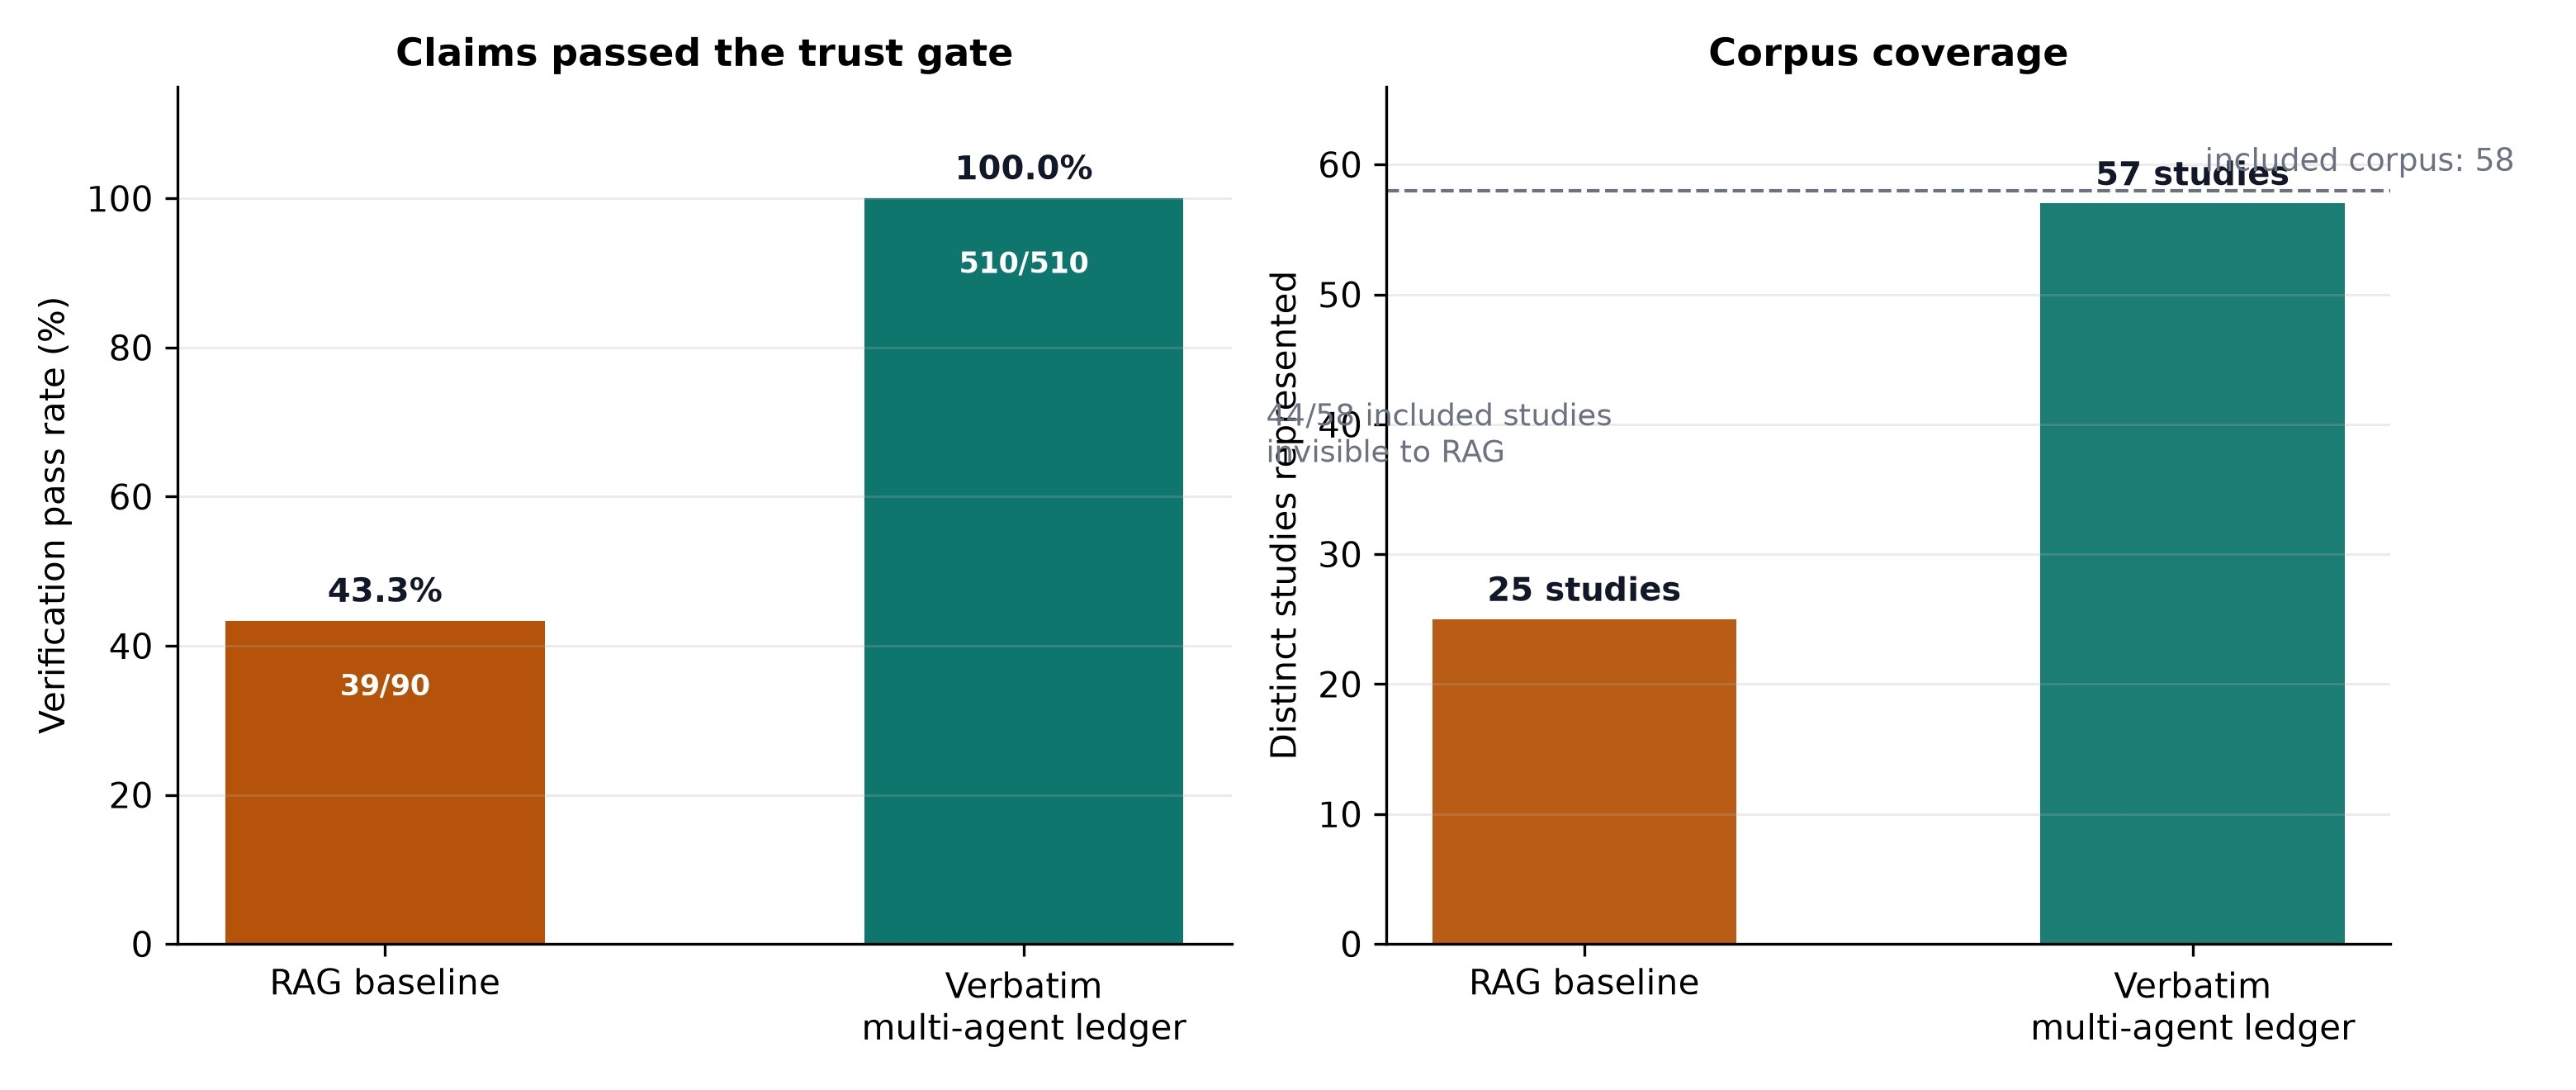
\includegraphics[keepaspectratio,alt={Figure 1 --- Head-to-head verification coverage.}]{../../synthesis/figures_d2/fig1_verification_versus_coverage.png}}
\caption{Figure 1 --- Head-to-head verification coverage.}
\end{figure}

The baseline verified fewer than half of its claims --- under its
\emph{own} self-referential entailment criterion, measured against the
very snippets that produced them, and it did so for only 8 of the 14
in-scope studies it covered. It under-covered the corpus in the same
breath: 44 of the 58 included studies never generated a single claim,
while one excluded study (SCI-000184) contributed 24\% of all RAG
claims. The verbatim pipeline, by contrast, covered all 57 claim-bearing
included studies with threshold-verified provenance (57 of 58 included
studies with at least one verified claim).

\subsubsection{3.2 Per-question rates and statistical
significance}\label{per-question-rates-and-statistical-significance}

\textbf{Table 2.} Per-question and pooled verification rates with Wilson
95\% confidence intervals.

{\def\LTcaptype{none} % do not increment counter
\begin{longtable}[]{@{}
  >{\raggedright\arraybackslash}p{(\linewidth - 10\tabcolsep) * \real{0.1364}}
  >{\raggedright\arraybackslash}p{(\linewidth - 10\tabcolsep) * \real{0.1364}}
  >{\raggedleft\arraybackslash}p{(\linewidth - 10\tabcolsep) * \real{0.1818}}
  >{\raggedleft\arraybackslash}p{(\linewidth - 10\tabcolsep) * \real{0.1818}}
  >{\raggedleft\arraybackslash}p{(\linewidth - 10\tabcolsep) * \real{0.1818}}
  >{\raggedleft\arraybackslash}p{(\linewidth - 10\tabcolsep) * \real{0.1818}}@{}}
\toprule\noalign{}
\begin{minipage}[b]{\linewidth}\raggedright
Arm
\end{minipage} & \begin{minipage}[b]{\linewidth}\raggedright
RQ1
\end{minipage} & \begin{minipage}[b]{\linewidth}\raggedleft
RQ2
\end{minipage} & \begin{minipage}[b]{\linewidth}\raggedleft
RQ3
\end{minipage} & \begin{minipage}[b]{\linewidth}\raggedleft
Pooled
\end{minipage} & \begin{minipage}[b]{\linewidth}\raggedleft
\end{minipage} \\
\midrule\noalign{}
\endhead
\bottomrule\noalign{}
\endlastfoot
RAG verified & 11/30 = 36.7\% & 14/30 = 46.7\% & 14/30 = 46.7\% & 39/90
= 43.3\% & \\
RAG Wilson 95\% CI & 21.9--54.5\% & 30.2--63.9\% & 30.2--63.9\% &
33.6--53.6\% & \\
Verbatim verified & 166/166 (100\%) & 132/132 (100\%) & 212/212 (100\%)
& 510/510 (100\%) & \\
Verbatim Wilson 95\% CI & 97.7--100\% & 97.2--100\% & 98.2--100\% &
99.3--100\% & \\
\end{longtable}
}

\textbf{Figure 2.} Per-research-question verification rates with Wilson
95\% CIs: the RAG baseline verifies 36.7\%/46.7\%/46.7\% (pooled floor
43.3\%); the verbatim pipeline verifies 100\% across RQ1--RQ3.

\begin{figure}
\centering
\pandocbounded{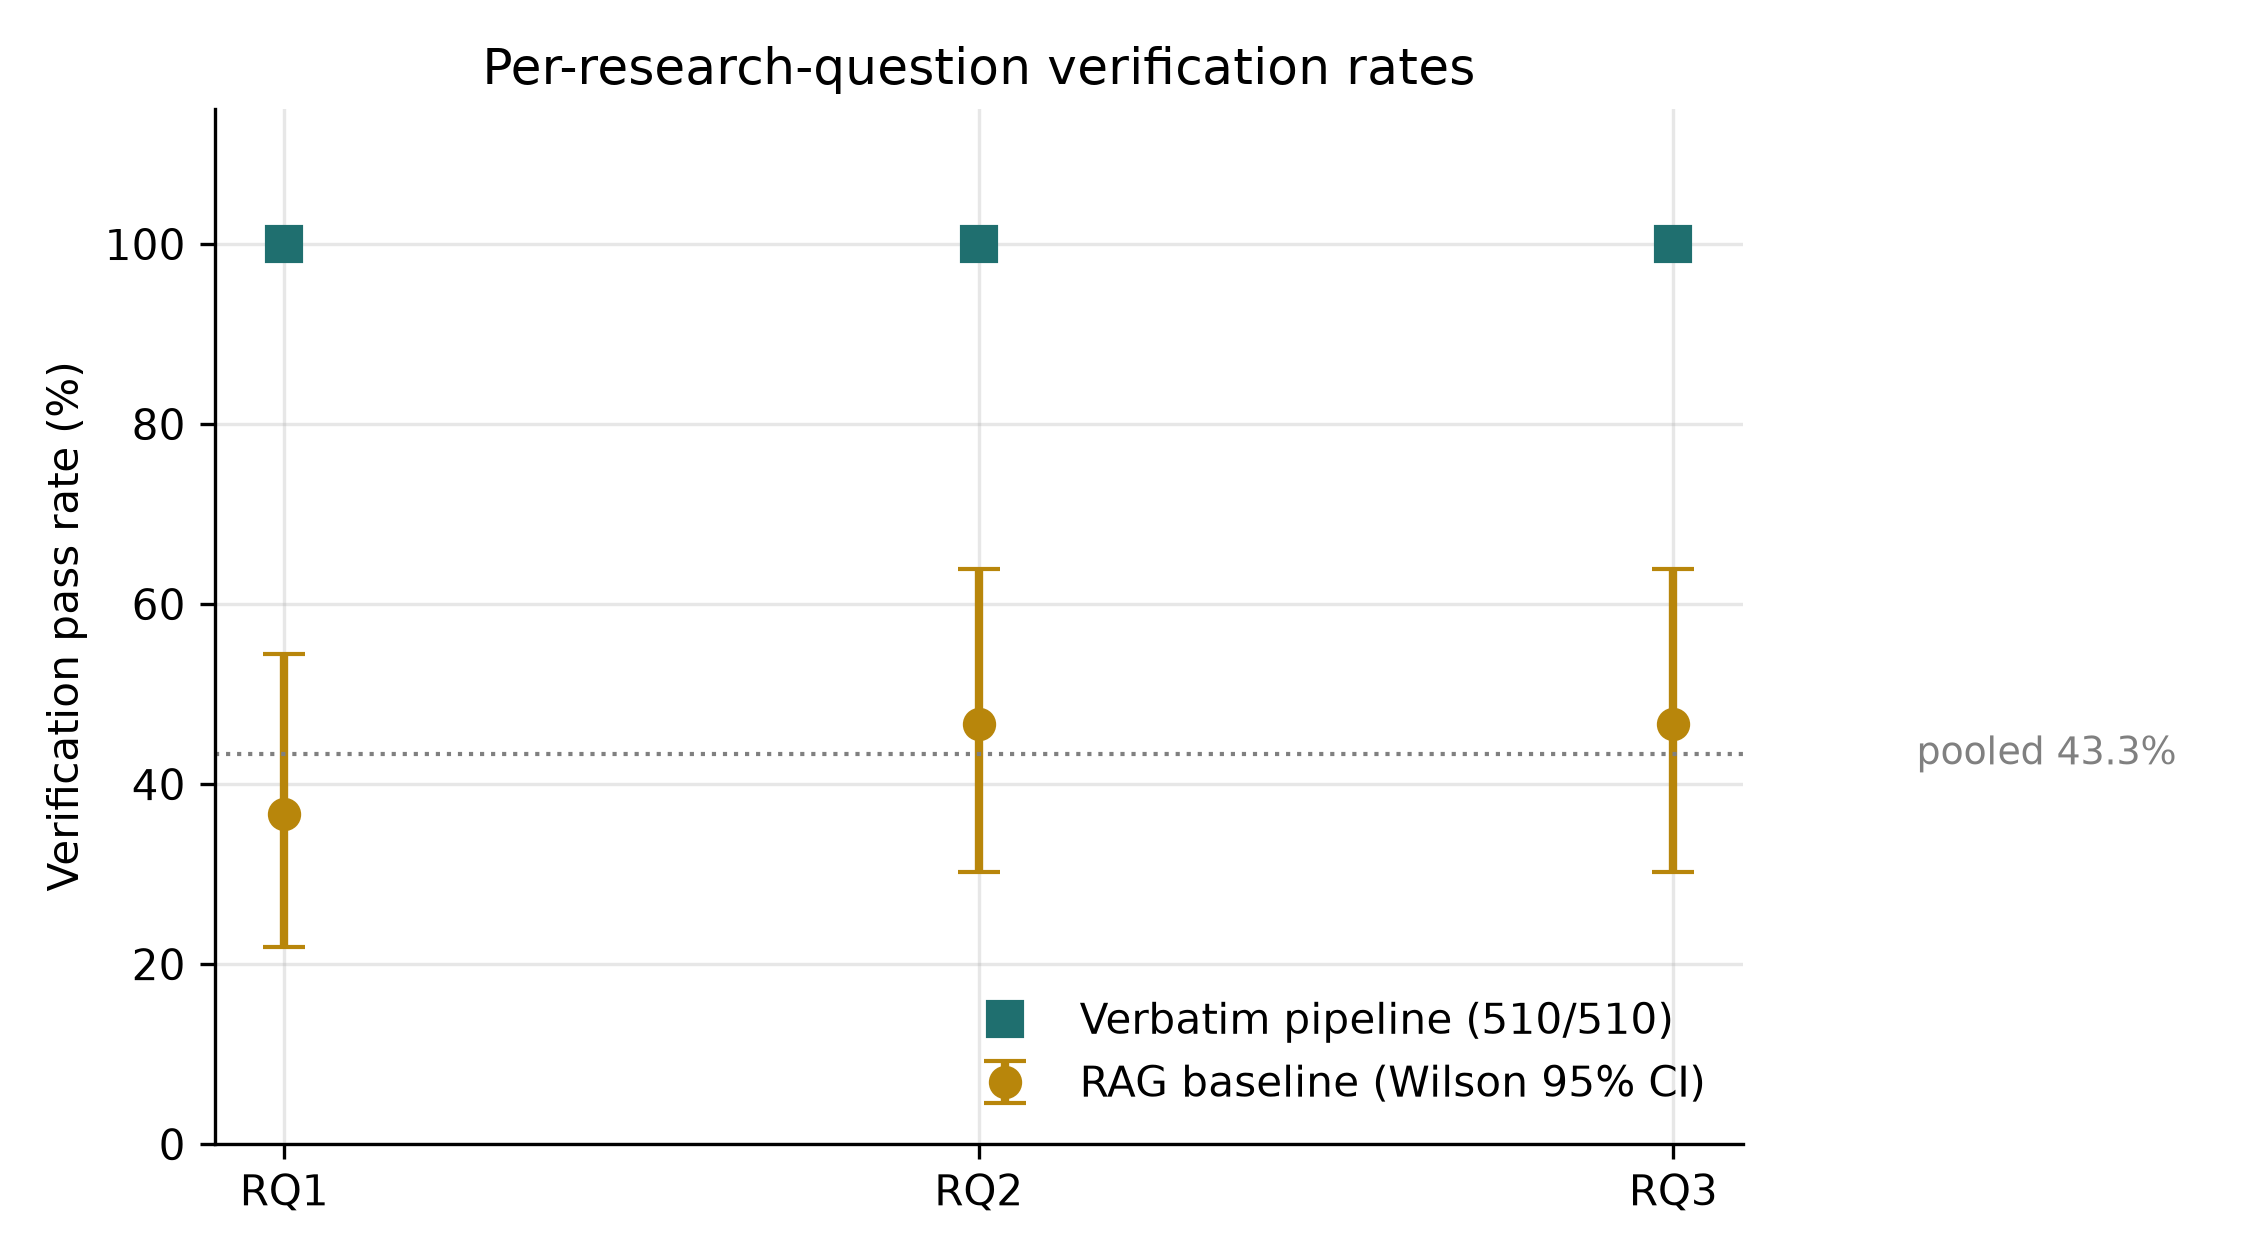
\includegraphics[keepaspectratio,alt={Figure 2 --- Per-research-question verification rates.}]{../../synthesis/figures_d2/fig4_per_rq_rates.png}}
\caption{Figure 2 --- Per-research-question verification rates.}
\end{figure}

The pooled contrast (39 vs 51; 510 vs 0) is decisive: one-sided Fisher
exact test, p ≈ 1.3 × 10⁻⁴⁹ (log₁₀ p ≈ −48.9). We report this as a
descriptive measure of the separation between arms rather than a
population inference: claims within a pipeline share generator context
and are not independent units, so the p-value cannot be read as a test
against a random-sampling null model (see §5).

\subsubsection{3.3 The verification repair
loop}\label{the-verification-repair-loop}

The verbatim gate acted as a live, strict signal rather than a post-hoc
stamp. Initial verification rejected \textbf{156 of 510} quotes
(30.6\%). Four repair iterations --- in which agents were fed the
precise failing quote and its source context --- reduced this first to
11, then, after re-casting those 11 residual light-paraphrase and
math-glyph artifacts (e.g., italic \texttt{*mIoU*} substrings) to exact
file substrings, to \textbf{0}. The ledger therefore reports
\textbf{510/510 (100\%)} verbatim-backed claims, with every failure
recorded against a \texttt{failure\_reason}
(\texttt{INSUFFICIENT\_COVERAGE}, \texttt{SOURCE\_TEXT\_NOT\_FOUND},
\texttt{MISSING\_QUOTE}) and versioned failure ledgers committed
alongside the data (\texttt{\_fails\_v3.json},
\texttt{\_fails\_v4.json}, \texttt{\_fails\_report.json}).

Two points about what the repair loop did and did not change. First,
iteration targeted the \emph{evidence quote}: repair agents were
required to re-locate the claim in the source text and return an exact
substring, not to rewrite the claim itself. The versioned failure
ledgers preserve the original failing quote and its coverage scores
(\texttt{idx}, \texttt{study\_id}, \texttt{rq\_id},
\texttt{claim\_text}, \texttt{quote}, \texttt{char\_cov},
\texttt{tok\_cov}) alongside the repaired outcome, so the before/after
is auditable. Second, the honest first-pass figure is \textbf{354/510
(69.4\%)}; the final 100\% is the endpoint of a tracked loop, and we
report both because they answer different questions --- how well the
pipeline grounds quotes initially, and whether the gate can be
\emph{fully} satisfied at all.

This is the point of a \emph{deterministic} gate: because the outcome of
each iteration is a database record rather than a model impression, the
repair loop is auditable version-by-version, and the final assertion ---
510/510 --- is externally checkable by anyone with the committed files,
including the possibility of re-simulating the pre-repair state from the
preserved failure ledgers.

\textbf{Figure 3.} The verification repair loop: 156/510 initial
failures (30.6\%) reduced to 11 after four repair iterations, then to 0
after re-casting light-paraphrase and math-glyph artifacts to exact file
substrings; each version's failure ledger is committed alongside the
data.

\begin{figure}
\centering
\pandocbounded{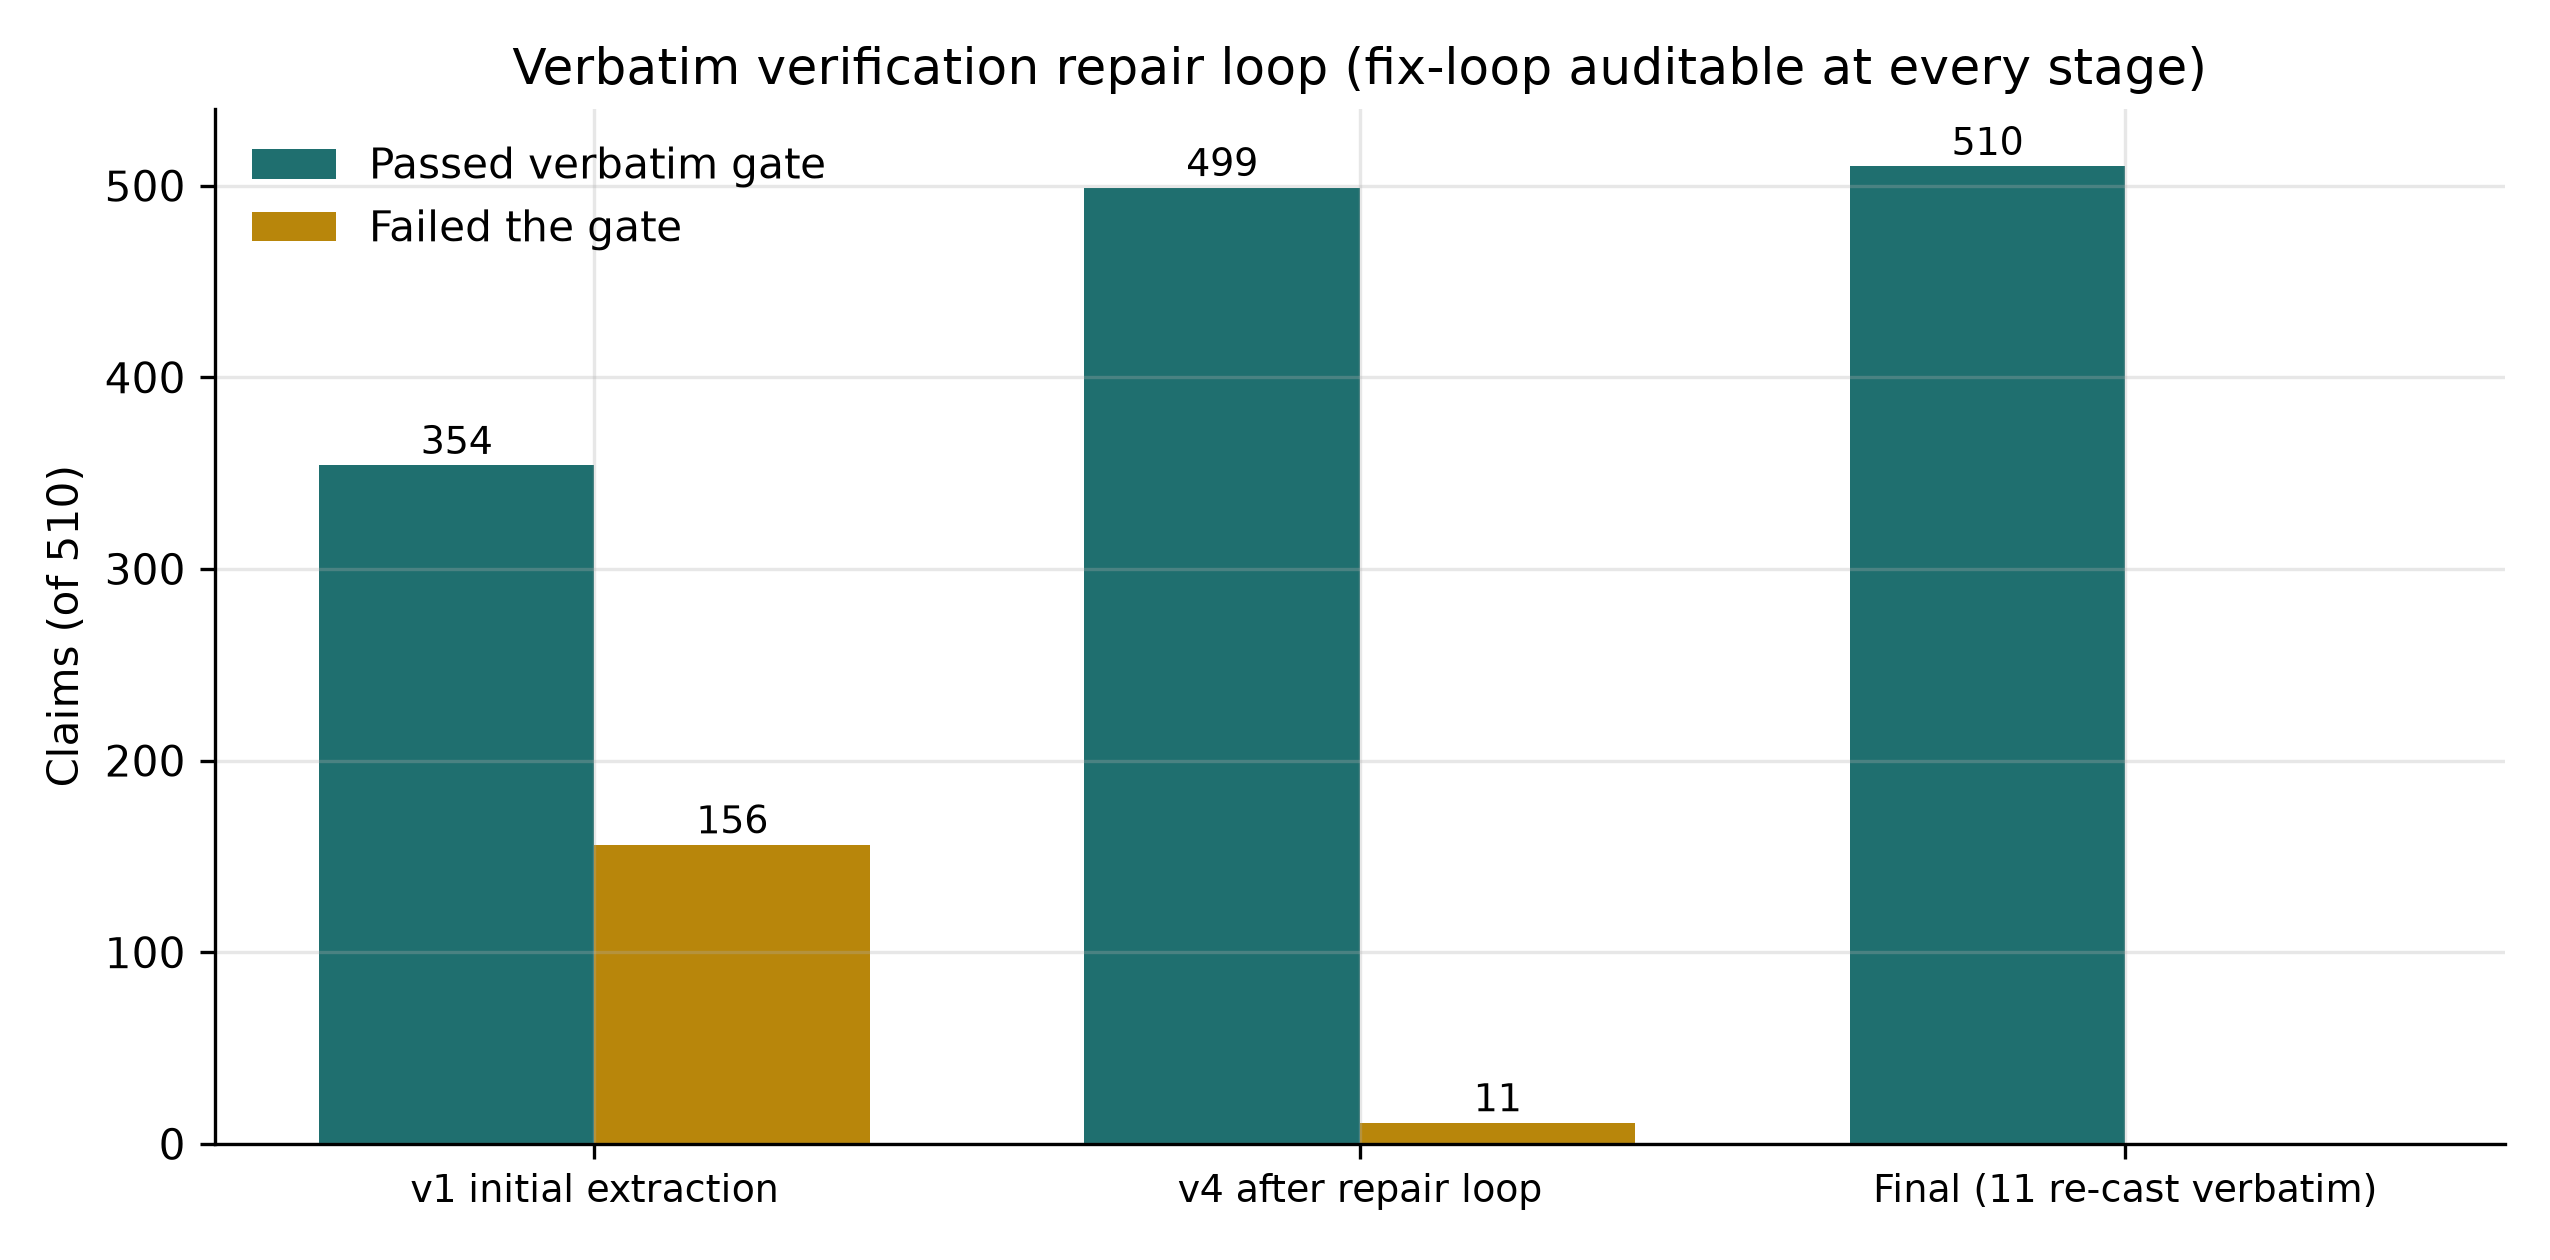
\includegraphics[keepaspectratio,alt={Figure 3 --- The verification repair loop.}]{../../synthesis/figures_d2/fig3_verification_repair_loop.png}}
\caption{Figure 3 --- The verification repair loop.}
\end{figure}

\subsubsection{3.4 Consensus structure and
scope}\label{consensus-structure-and-scope}

Consensus clustering sharpened rather than flattened the evidence. The
verbatim ledger produced \textbf{95 clusters with 7 active debates} ---
clusters containing directly conflicting claims from different studies
--- whereas the RAG baseline, with a tenth of the claims restricted to
top-30 retrieval, produced \textbf{20 clusters and zero debates}. Debate
structure is precisely what retrieval-association cannot see:
recognizing genuine disagreement between two passages requires reading
both, not retrieving the closer of two.

\textbf{Figure 4.} Corpus-scope discipline and debate structure: the RAG
baseline drew on 18 screened-out extractions in its index (citing 11
non-included studies, dominated by SCI-000184 with 22/90 claims) and
left 44 included studies with zero claims; the verbatim ledger,
restricted to the 58 included studies, surfaced 95 clusters including 7
active debates.

\begin{figure}
\centering
\pandocbounded{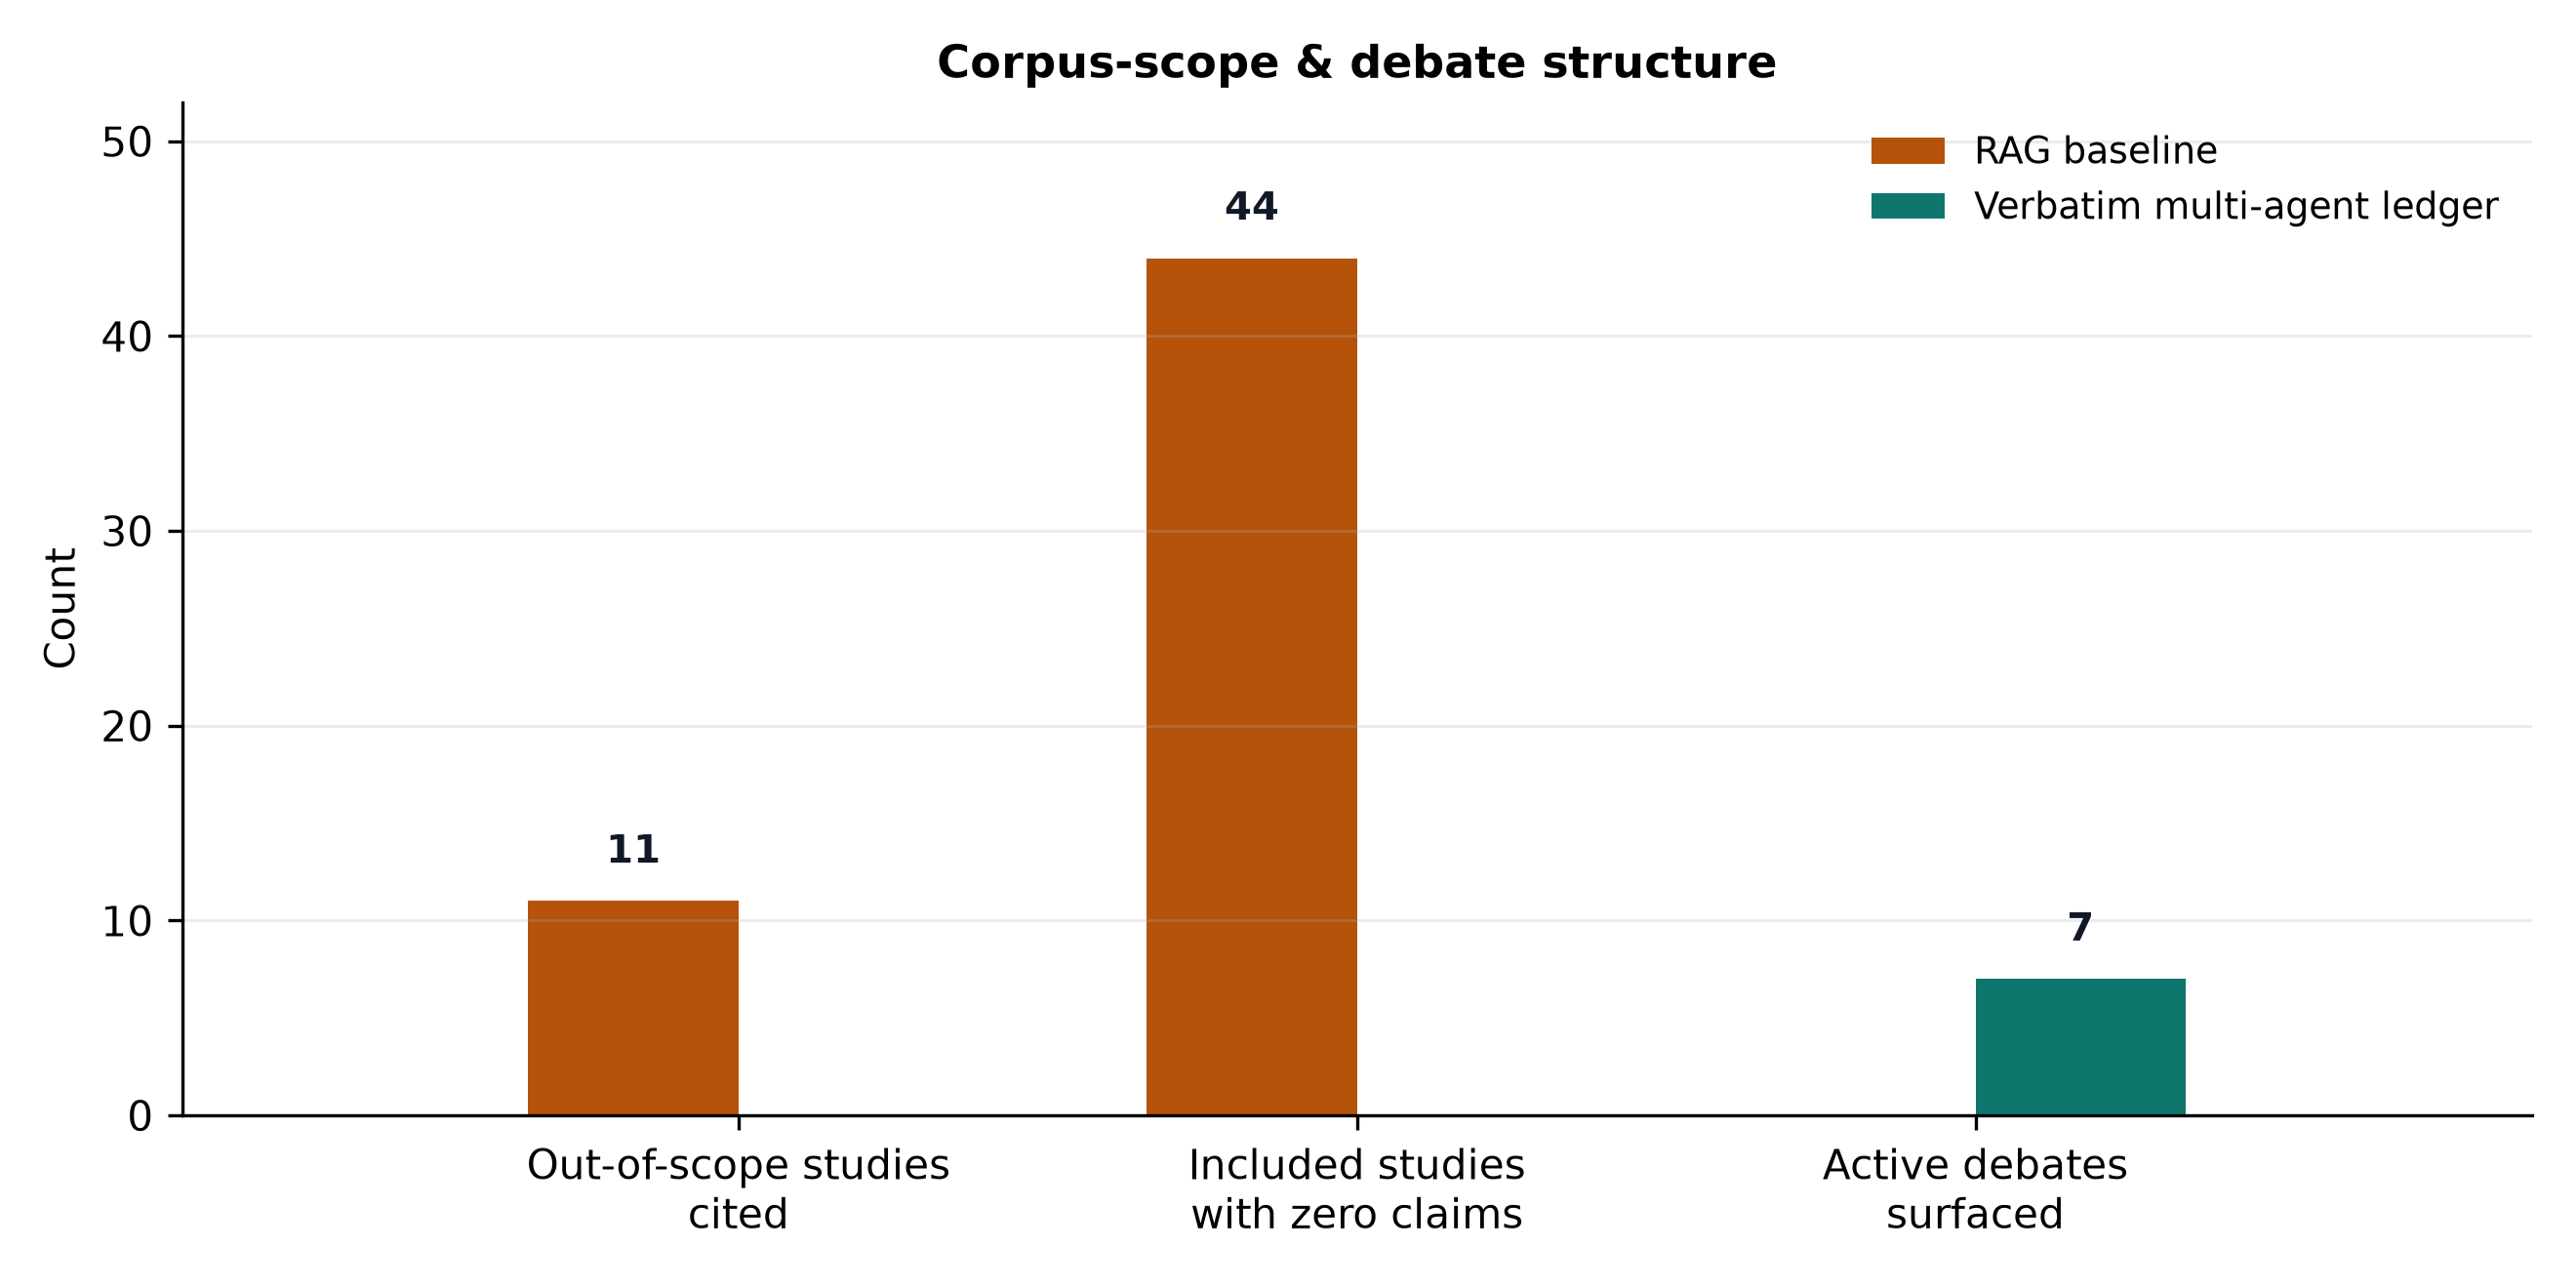
\includegraphics[keepaspectratio,alt={Figure 4 --- Corpus-scope discipline and debate structure.}]{../../synthesis/figures_d2/fig2_scope_and_debates.png}}
\caption{Figure 4 --- Corpus-scope discipline and debate structure.}
\end{figure}

\subsection{4. Discussion}\label{discussion}

Three findings deserve emphasis, in increasing order of importance.

\textbf{Retrieval restriction is simultaneously a coverage failure and a
contamination failure.} The top-30 window excluded 44 of 58 included
studies entirely, while the pre-scoping index silently served 11
excluded studies into citation space. Neither pathology is fixable by
tuning \texttt{k}: window tightness and index purity are separate
decisions, and the second --- scope enforcement --- is the one that
matters for trust. Every RAG claim is a bet that the retrieval window
contained the right evidence and that the index contained \emph{only}
approved evidence; our baseline lost that bet on both counts.

\textbf{Verbatim is not entailment.} Entailment asks whether a claim is
consistent with a retrieval context; verbatim asks whether the claim's
exact wording exists in an approved source. These answer different
questions, and the first is the one that hallucination exploits. A
system that says ``the snippet supports this'' is not saying ``this
sentence appears in the paper.'' The 43.3\% baseline figure understates
the problem rather than overstating it --- it is the RAG system's
self-report against its own snippets, and it is already low enough to
disqualify the output from evidence synthesis intended for peer review.

\textbf{Determinism turns verification into an audit rather than a
judgment.} Coverage thresholds, character windows, and token 6-grams are
all open parameters; anyone can rerun the gate and re-derive 510/510
from the committed quotes. The repair loop iterated against a fixed,
versioned gate until all failures were resolved, and each iteration is
recorded for external audit. An LLM-as-a-judge system, by contrast, can
neither report exact failure reasons nor prove that its verdict would be
stable tomorrow.

We also want to be candid about what this comparison does and does not
show. The RAG arm is evaluated by \emph{its own} criterion, because its
schema carries no quotes for us to check; 43.3\% is therefore the
system's self-reported verification rate, not a verdict we imposed on
it. Second, the two pipelines share no claims, and claims within a
pipeline share generator context, so the Fisher p-value is a descriptive
statement of effect size rather than a population inference --- a point
reviewers will rightly probe.

\subsubsection{4.1 Prior work, in one
paragraph}\label{prior-work-in-one-paragraph}

The surrounding literature supports both the diagnosis and the remedy.
Citation-fabrication studies repeatedly find low existential ceilings
that post-hoc validation only partially restores {[}1{]}{[}2{]}.
Evaluations of screening and extraction tools converge on a different
gap --- that performance is unstable across runs and prompts, and that
similarity-based scoring (ROUGE, BERTScore, BLEU) fails to track human
judgment {[}3{]}{[}4{]}. Several system papers adopt retrieval
grounding, synthesis-style consensus, or provenance journals
individually {[}2{]}{[}5{]}; this study is most directly comparable to
those, but it combines scope enforcement, verbatim grounding, versioned
repair, consensus clustering, and continuous trust monitoring in a
single pipeline --- and measures a homogeneous RAG baseline against the
same corpus under the same screening conditions.

\subsection{5. Limitations}\label{limitations}

\begin{itemize}
\tightlist
\item
  \textbf{Single corpus.} The comparison is confined to one domain (AI
  research harnesses, 58 studies), of which a substantial share are
  arXiv preprints (31 of 64 extractions cite arXiv). Verbatim matching
  is applied to both preprint and publisher-rendered text here, but the
  magnitude of the effect --- and the balance of failure types --- could
  differ in other fields or document mixes. Replication is required
  before generalizing the magnitude, though not the direction, of the
  effect.
\item
  \textbf{Incomplete full-text coverage.} Twelve included studies
  contributed abstract-only claims (17 of 510); one (SCI-000147)
  contributed none.
\item
  \textbf{Claim-level statistics are descriptive.} Claims are generated
  by a small number of agents and are not independent observational
  units; the Fisher test in §3.2 is reported and must be read as an
  effect-size descriptor, not a population inference. The study-level
  figures (8 of 14 for RAG; 57 of 58 for the verbatim pipeline) are the
  more conservative summary of the same contrast.
\item
  \textbf{Repair-loop edits are quote-level only.} Iteration re-located
  exact substrings rather than rewriting claims, but a residual risk
  remains that an exact substring may not perfectly preserve the claim's
  intended semantic emphasis; the preserved failure ledgers allow
  reviewers to judge this case by case.
\item
  \textbf{Verbatim is a necessary, not sufficient, condition.} A
  quote-bearing claim is grounded, but the quote may not be
  representative of its source, and claim-to-quote semantic completeness
  is only partially covered by RQ tagging and stance fields.
\item
  \textbf{Clustering choices.} Consensus used a single embedding model
  and a hand-set threshold (θ = 0.40).
\item
  \textbf{Baseline parameters.} Top-30 retrieval and the entailment
  heuristic are reasonable defaults chosen in advance; they are not an
  adversarial worst case for RAG.
\item
  \textbf{Screeners are AI.} Screening decisions are aggregate judgments
  of four agents with fair agreement, adjudicated at deadlock; they are
  not human-gold-standard in origin.
\end{itemize}

\subsection{6. Conclusion}\label{conclusion}

Evidence synthesis is only credible for publication when each claim is
bound to a machine-verified quote from an approved source at a stated,
reproducible coverage threshold (≥0.90 glyph-normalized coverage on
char-window or token 6-gram alignment). On one identical corpus, a
retrieval-associative baseline verified 43.3\% of its own claims and
drew on content outside the included set; a verbatim pipeline reached
100\% with zero contamination, a versioned repair trail, and a richer
consensus structure that exposed real scientific disagreement. We
recommend verbatim claim verification as the default trust gate for
LLM-assisted systematic review, corpus-scope enforcement as its
precondition, and consensus-aware trust weighting and append-only audit
as the complementary layers around it.

\subsection{7. Declarations}\label{declarations}

\begin{itemize}
\tightlist
\item
  \textbf{Competing interests}: none declared. The generating harness
  was itself the object of study; the surface area of its own tooling
  was not part of the evaluated corpus.
\item
  \textbf{Data availability}: all artifacts are committed in the
  \texttt{nexus-scholar-harness} repository under
  \texttt{workspaces/ai-research-harnesses-trust/}: verbatim ledger
  \texttt{synthesis/claims.json} (510 claims, each with a
  machine-verified quote), \texttt{synthesis/rag\_baseline/} (RAG arm),
  \texttt{synthesis/consensus.json\textbar{}md} (95 clusters),
  \texttt{phase4/*} (trust streams), and the append-only
  \texttt{audit/journal.jsonl} (69 events).
\item
  \textbf{Code availability}: the verifier is open source
  (\texttt{scholar-verify-kit}, module
  \texttt{scholar\_verify.verbatim}); figures regenerate from
  \texttt{scripts/build\_d2\_figures.py}; every headline number is
  recomputed and asserted against the committed ledgers by
  \texttt{scripts/reproduce\_d2\_stats.py}
  (\texttt{uv\ run\ python\ scripts/reproduce\_d2\_stats.py}), which
  exits non-zero on any mismatch and writes an audit report to
  \texttt{synthesis/figures\_d2/stats\_audit.md}.
\item
  \textbf{Author contributions}: both authors contributed equally to
  conceptualization, methodology, and writing; S.Z. is the corresponding
  author.
\item
  \textbf{Ethics statements}: not applicable (no human subjects; review
  of published literature).
\end{itemize}

\subsection{References}\label{references}

{[}1{]} Zhao, C., Tang, Y., \& Qian, Y. \emph{Do Deployment Constraints
Make LLMs Hallucinate Citations? An Empirical Study across Four Models
and Five Prompting Regimes.} arXiv preprint, 2026. (Workspace:
SCI-000144.) Verbatim-ledger metrics: max citation-existence rate 0.475
across 17,443 citations; manual audit agreement 0.63; 16/35
``Unresolved'' labels actually fabricated.

{[}2{]} Asai, A., He, J., Shao, R., Shi, W., Singh, A., Chang, J. C.,
Lo, K., Soldaini, L., Feldman, S., D'Arcy, M., Wadden, D., Latzke, M.,
Sparks, J., Hwang, J. D., Kishore, V., Tian, M., Ji, P., Liu, S., Tong,
H., Wu, B., Xiong, Y., Zettlemoyer, L., Neubig, G., Weld, D. S., Downey,
D., Yih, W.-t., Koh, P. W., \& Hajishirzi, H. \emph{OpenScholar:
Synthesizing Scientific Literature with Retrieval-augmented LMs.}
arXiv:2411.14199, 2024. DOI: 10.48550/arxiv.2411.14199. (Workspace:
SCI-000159.) Verbatim-ledger metrics: non-retrieval LLMs fabricate
78--98\% of cited papers; OpenScholar-8B zero hallucinated papers.

{[}3{]} Ha, H. H., Favre, B., \& Portet, F. \emph{MedMeta: A Benchmark
for LLMs in Synthesizing Meta-Analysis Conclusion from Medical Studies.}
arXiv:2605.09661, 2026. (Workspace: SCI-000127.) Verbatim-ledger
metrics: BERTScore rates false N-RAG conclusions as semantically
equivalent to G-RAG.

{[}4{]} Schmidt, L., Hair, K., Graziosi, S., Campbell, F., Kapp, C.,
Khanteymoori, A., Craig, D., Engelbert, M., \& Thomas, J.
\emph{Exploring the use of a Large Language Model for data extraction in
systematic reviews: a rapid feasibility study.} arXiv preprint, 2024.
(Workspace: SCI-000108.) Verbatim-ledger metrics: BLEU/ROUGE results
``not meaningful'' against human assessment.

{[}5{]} Lewis, P., Perez, E., Piktus, A., Petroni, F., Karpukhin, V.,
Goyal, N., Küttler, H., Lewis, M., Yih, W.-t., Rocktäschel, T., Riedel,
S., \& Kiela, D. \emph{Retrieval-Augmented Generation for
Knowledge-Intensive NLP Tasks.} Advances in Neural Information
Processing Systems 33, 9459--9474, 2020. arXiv:2005.11401; DOI:
10.48550/arXiv.2005.11401.

{[}6{]} Fleiss, J. L. \emph{Measuring nominal scale agreement among many
raters.} Psychological Bulletin, 76(5): 378--382, 1971. DOI:
10.1037/h0031619.

{[}7{]} Reimers, N., \& Gurevych, I. \emph{Sentence-BERT: Sentence
Embeddings using Siamese BERT-Networks.} Proceedings of EMNLP-IJCNLP
2019, pp.~3982--3992, 2019. DOI: 10.18653/v1/D19-1410.

{[}8{]} Whiting, P. F., Rutjes, A. W. S., Westwood, M. E., et
al.~\emph{QUADAS-2: A Revised Tool for the Quality Assessment of
Diagnostic Accuracy Studies.} Annals of Internal Medicine, 155(8):
529--536, 2011. DOI: 10.7326/0003-4819-155-8-201110180-00009.

{[}9{]} Wolff, R. F., Moons, K. G. M., Riley, R. D., et
al.~\emph{PROBAST: A Tool for Assessing the Risk of Bias and
Applicability of Prediction Model Studies.} Annals of Internal Medicine,
170(1): 51--58, 2019. DOI: 10.7326/M18-1376.

{[}10{]} Landis, J. R., \& Koch, G. G. \emph{The measurement of observer
agreement for categorical data.} Biometrics, 33(1): 159--174, 1977. DOI:
10.2307/2529310.

{[}11{]} Zhang, T., Kishore, V., Wu, F., Weinberger, K. Q., \& Artzi, Y.
\emph{BERTScore: Evaluating Text Generation with BERT.} ICLR 2020.
arXiv:1904.09675; DOI: 10.48550/arXiv.1904.09675.

{[}12{]} Lin, C.-Y. \emph{ROUGE: A Package for Automatic Evaluation of
Summaries.} In Text Summarization Branches Out: Proceedings of the
ACL-04 Workshop, pp.~74--81. Barcelona: ACL, 2004. (ACL Anthology:
W04-1013.)

{[}13{]} Page, M. J., McKenzie, J. E., Bossuyt, P. M., Boutron, I.,
Hoffmann, T. C., Mulrow, C. D., et al.~\emph{The PRISMA 2020 statement:
an updated guideline for reporting systematic reviews.} BMJ, 372: n71,
2021. DOI: 10.1136/bmj.n71.

{[}14{]} Tricco, A. C., Lillie, E., Zarin, W., O'Brien, K. K.,
Colquhoun, H., Levac, D., et al.~\emph{PRISMA Extension for Scoping
Reviews (PRISMA-ScR): Checklist and Explanation.} Annals of Internal
Medicine, 169(7): 467--473, 2018. DOI: 10.7326/M18-0850.

\end{document}
